%
%                  Politecnico di Milano
%
%         Student: Caravano Andrea, Cantele Alberto
%            A.Y.: 2024/2025
%
%   Last modified: 05/04/2025
%
%     Description: Internet of Things: Challenge n. 2
%                  Packet captures analysis report
%

\documentclass[a4paper,11pt]{article} % tipo di documento
\usepackage[T1]{fontenc} % codifica dei font
\usepackage[utf8]{inputenc} % lettere accentate da tastiera
\usepackage[english,italian]{babel} % lingua del documento
\usepackage{lipsum} % genera testo fittizio
\usepackage{url} % per scrivere gli indirizzi Internet e/o di riferimento nella pagina

\usepackage[hidelinks]{hyperref} % per modificare il comportamento dei collegamenti ipertestuali (+ leva colore attorno)

\usepackage[margin=0.7in]{geometry} % margine di pagina

\usepackage{graphicx} % per inserire immagini

\usepackage[outputdir=../auxil]{minted} % per colorazione automatica del codice (installare pygments da Homebrew)
% \usepackage{pythonhighlight} % per Python

\usepackage{fancyhdr}
\usepackage{textcomp}
\usepackage{siunitx} % per gestione intestazione e piè di pagina

\usepackage{listings} % per frammenti di codice
\usepackage{xcolor} % per colori personalizzati frammenti di codice

\usepackage{tcolorbox} % per riquadrature di vario colore

\hypersetup{ % metadati di titolo e autore nel PDF
    pdftitle={Internet of Things: Challenge n. 2},
    pdfauthor={Andrea Caravano, Alberto Cantele}
}

\setlength{\parindent}{0pt} % rimuove l'indentazione del testo

% Colori per frammenti di codice
\definecolor{codegreen}{rgb}{0,0.6,0}
\definecolor{codegray}{rgb}{0.5,0.5,0.5}
\definecolor{codepurple}{rgb}{0.58,0,0.82}
\definecolor{backcolour}{HTML}{F5F5F5}

\lstdefinestyle{code_fragments}{
    backgroundcolor=\color{backcolour},
    commentstyle=\color{codegreen},
    keywordstyle=\color{magenta},
    numberstyle=\tiny\color{codegray},
    stringstyle=\color{codepurple},
    basicstyle=\ttfamily\footnotesize, % dimensione del testo
    breakatwhitespace=false,
    breaklines=true,
    captionpos=b,
    keepspaces=true,
    numbers=left,
    numbersep=5pt,
    showspaces=false,
    showstringspaces=false,
    showtabs=false,
    tabsize=2,
    frame=single, % Bordo singolo attorno al codice
    framerule=0.5pt, % Spessore del bordo
    framesep=2pt, % Distanza dal testo al bordo
    rulecolor=\color{gray} % Colore del bordo
}

% Imposizione stile dei frammenti di codice
\lstset{style=code_fragments}

\setminted{ % si può impostare il linguaggio specifico con \setminted[JSON] ad esempio
    linenos=true,
    breaklines=true,
    encoding=utf8,
    fontsize=\small,
    bgcolor=backcolour,
    frame=lines
}

\tcbset{ % impostazioni per riquadrature
    colback=gray!20,
    colframe=black,
    boxrule=0.5pt
}

\begin{document}
    \pagestyle{fancy}
    \fancyhead{}\fancyfoot{}
    \fancyhead[L]{\textbf{Internet of Things: Challenge n. 2}}
    \fancyhead[R]{Andrea Caravano, Alberto Cantele}
    \fancyfoot[C]{\thepage}

    \title{\textbf{Internet of Things}\\Challenge n. 2: Packet captures analysis}
    \author{Andrea Caravano, Alberto Cantele}
    \date{Academic Year 2024--25}
    \maketitle


    \section{Implementation and design choices}\label{sec:implementation-and-design-choices}

    All the question have been answered by implementing a \textsc{Python} notebook, correlated by a group of custom functions, declared in a dedicated library, to ease readability and clarity of the overall structure.

    Each question has its own separate space.
    The only common parts to all questions are situated right on top of the notebook, where libraries import and constants declarations are placed.

    In the following, all questions and related resolution strategies are described, providing a deeper explanation to the most meaningful points.

    \subsection{Optionally: a Docker container}\label{subsec:optionally:-a-docker-container}

    The \textsc{PyShark} library, used for parsing of the packet capture file, requires installation of \textsc{tshark} on the local machine, being implemented as a wrapper to it.

    Therefore, to provide a common abstraction layer, a specifically crafted \textsc{Dockerfile} is included in the repository, providing all the most common \textsc{Jupyter notebooks} requirements, alongside \textsc{tshark}.

    When built, it can be used to serve as an interpreter for the project, integrating it with the embedded \textsc{Python Conda} environment.


    \section{Question n. 1}\label{sec:question-n.-1}
    How many \textbf{different} Confirmable PUT requests obtained an unsuccessful response from the local CoAP server?

    \medskip

    The resolution strategy is roughly described as follows.

    \begin{itemize}
        \item Filter \textsc{CoAP CONfirmable PUT} requests, directed to the local \textsc{CoAP Server} (localhost/loopback address)

        This translates to the following filter:

        \texttt{coap and coap.type == 0 and coap.code == 3 and (ip.dst == 127.0.0.1 or ipv6.dst == ::1)}

        With type 0 being the one for \textsc{CONfirmable} messages and code 3 being the one for \textsc{PUT} requests.

        We are then filtering those directed to the local \textsc{CoAP Server}, using both \textsc{IPv4} and \textsc{IPv6} notation (\texttt{127.0.0.1} or \texttt{::1}, corresponding to the loopback interface, managed by the operating system kernel itself).
        \item A uniquely hashed data structure (a set) stores a copy of the token identifier for each packet: this is useful to match a couple of request and response messages, as we are asked to elaborate on responses to the requests we filtered earlier.
        \item Filter CoAP responses coming from the local \textsc{CoAP Server} (localhost/loopback address), opposite with respect to the case shown before, naturally, having a response code included in the group of client/server-side errors (similar to the HTTP 400\ --\ 500 group).

        This translates to the following filter:

        \texttt{coap and coap.type == 2 and coap.code >= 128 and coap.code <= 165 and (ip.src == 127.0.0.1 or ipv6.src == ::1)}

        With type 2 being the type for \textsc{Acknowledgements} and code 128 and 165 being the boundaries of client/server-side errors response codes.
        \item For each token found among this second group of filtered packets, inclusion in the set of tokens found earlier is determined.
        \item If the token belongs to the set, it matches the criteria and therefore the final counter of matches is incremented.
    \end{itemize}

    The number of \textbf{matches found} for the criteria of \textbf{Question n. 1 is 22}.


    \section{Question n. 2}\label{sec:question-n.-2}
    How many CoAP \textbf{resources} in the \textbf{coap.me} public server received the same number of \textbf{unique} Confirmable and Non Confirmable GET requests?

    Assuming a resource receives \textbf{$X$} \underline{different} CONFIRMABLE requests and \textbf{$Y$} \underline{different} NONCONFIRMABLE GET requests, how many resources have $X = Y$, with $X > 0$?

    \subsection{A note on DNS symbolic names resolution}\label{subsec:a-note-on-dns-symbolic-names-resolution}

    \texttt{coap.me} is a symbolic name, that needs to be translated (resolved) using the \textsc{DNS} protocol.

    The most reasonable assumption for our case, is that the level of detail present in the packet capture files, matches, at least, the one needed to reconstruct the entire traffic flow up to the \textsc{DNS} resolution of the public server address.

    The address therefore used to refer to the \texttt{coap.me} server (and later to the \textsc{HiveMQ} and \textsc{Mosquitto} brokers) are the ones contained in the \textsc{DNS} answers included in the packet capture.

    Resolving those addresses locally or, in the best approximation possible, geographically distributing the query, is not equivalent.

    The \textsc{DNS} protocol is very often used as a secondary load balancing measure, providing different answers in response to the congestion level of the system, geographical position of the client and a great variety of many more tunable parameters, chosen by the service provider and its internal processes evaluation.

    Relying on the resolution provided by the capture itself is, in the end, the best approach.

    Underlying assertion in the following questions is that the number of addresses found as resolutions of the provided symbolic name, is greater (or equal) than 1.

    \medskip

    The resolution strategy is roughly described as follows.

    \begin{itemize}
        \item Gather DNS answers to the \texttt{coap.me} symbolic name query, \hyperref[subsubsec:dns-resolution-python]{through a custom function designed to ease re-use among the multiple questions having a symbolic name resolution in common}, \hyperref[sec:question-n.-2]{as described}.

        In our case, the set of resulting addresses is just composed of the \textsc{IPv4} one: \texttt{134.102.218.18}.
        \item Filter all \textsc{CoAP GET Requests}, that will then be parsed deeply.

        This translates to the following filter:

        \texttt{coap.code == 1}

        With 1 being the code for \textsc{GET Requests}.

        \item Create a pair of dictionaries (a hashmap-like data structure), allowing any value as key or inner content.
        In our case, the \textsc{URI} destination will be the key for all structures.
        \item Filter packets destined to one of the \texttt{coap.me} addresses resolved earlier.
        \item Distinguish among \textsc{CONfirmable} and \textsc{NON-confirmable} requests.

        For each new \textsc{URI} found, an entry is created in the dictionaries, storing a set of all of the tokens that requested the specific \textsc{URI} and counting them.

        In our case, the matching set of resources found are:

        \begin{center}
            \begin{tabular}{|c|c|c|c|}
                \hline
                Resource URI    & CONfirmable requests & NON-confirmable requests \\
                \hline
                /3              & 4                    & 0                        \\
                \hline
                /weird44        & 1                    & 2                        \\
                \hline
                /4              & 2                    & 1                        \\
                \hline
                /large          & 1                    & 1                        \\
                \hline
                /validate       & 1                    & 1                        \\
                \hline
                /secret         & 1                    & 1                        \\
                \hline
                /location-query & 1                    & 0                        \\
                \hline
                /location1      & 1                    & 0                        \\
                \hline
                /hello          & 1                    & 0                        \\
                \hline
                /weird          & 2                    & 3                        \\
                \hline
                /weird33        & 3                    & 1                        \\
                \hline
                /5              & 1                    & 0                        \\
                \hline
                /multi-format   & 2                    & 0                        \\
                \hline
                /sink           & 1                    & 3                        \\
                \hline
                /weird333       & 0                    & 2                        \\
                \hline
                /broken         & 0                    & 1                        \\
                \hline
                /separate       & 0                    & 1                        \\
                \hline
                /large-create   & 0                    & 1                        \\
                \hline
            \end{tabular}
        \end{center}
        \item The two resulting sets of resources (\textsc{URI} identifiers) are intersected and, for common resources, a comparison among seen tokens in both cases (therefore, unique \textsc{GET Requests}) is performed, leading to the final result.
    \end{itemize}

    The number of \textbf{matches found} for the criteria of \textbf{Question n. 2 is 3}.


    \section{Question n. 3}\label{sec:question-n.-3}
    How many \textbf{different} MQTT clients subscribe to the \textbf{public broker HiveMQ} using multi-level wildcards?

    \medskip

    The resolution strategy is roughly described as follows.
    \begin{itemize}
        \item Gather \textsc{DNS} answers to the \texttt{broker.hivemq.com} symbolic name query, \hyperref[subsubsec:dns-resolution-python]{through a custom function designed to ease re-use among the multiple questions having a symbolic name resolution in common}, \hyperref[sec:question-n.-2]{as described}.

        In our case, the set of resulting addresses is composed by the \textsc{IPv4} triple: \texttt{35.158.34.213}, \texttt{35.158.43.69}, \texttt{18.192.151.104}.
        \item Filter \textsc{MQTT Subscribe} packets having an interest declaration (topic) matching the regular expression “.*\#”.

        The regular expression implements a simple Finite State Automata with initial state every possible character in the alphabet (the content of the string) and reaching a final state only when encountering a multi-level wildcard (\#).

        Then, it is necessary to ensure the string does not match the pattern “\#.+” meaning that after the wildcard (\#) any character follows, which describes an invalid behaviour.

        In practice, the regular expression matches every string containing a \# at (only) the last position.

        The corresponding Finite State Machine implementing the regular pattern is the following.

        \begin{center}
            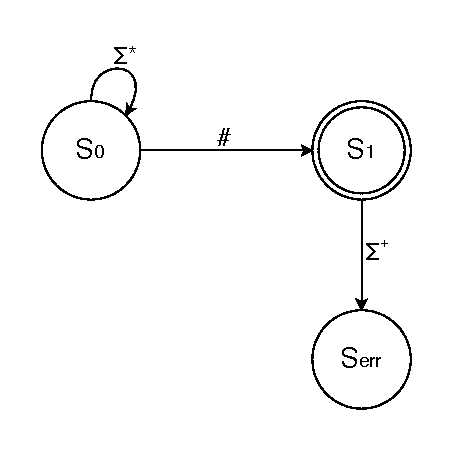
\includegraphics[width=6cm]{../res/FSA_Q3}
        \end{center}

        This translates to the following filter:

        \texttt{mqtt and mqtt.msgtype == 8 and mqtt.topic matches ".*\#" and !mqtt.topic matches "\#.+"}

        With 8 being the \textsc{SUBSCRIBE} message type.

        Filtering deeply on the HiveMQ broker addresses as destination yields to 6 packets left to analyze.
        \item For each packet destined to the HiveMQ broker, a distinctive element for each client should be found.

        Following the assumption that each client uses a different socket pair during the entire lifetime of the packet capture, we could directly bind a client to its socket.

        \label{description-clientids}
        However, a more general approach relies on MQTT's client ids, being uniquely defined for each client connected to a broker.

        In this case, the broker is common among all clients, so we should trace the ID of each client, using its most-recent \textsc{CONNECT} message, that embeds it (and related \textsc{CONNECT ACK}).

        Note that, since the client ID may be empty or replicated, a reasonable precaution is to store both details.

        Further details of the implementation for the custom-crafted client ids derivation function, are \hyperref[subsubsec:mqtt-clientid-python]{provided in the related section}.
        \item The number of matching packets will be the length of the resulting unique client identifiers and socket pairs count, made possible by a supporting sorted list data structure.

        A manual inspection on the 6 packets mentioned earlier, aimed in particular at the socket definitions of all clients, confirms the outcome.
    \end{itemize}

    The number of \textbf{matches found} for the criteria of \textbf{Question n. 3 is 4}.


    \section{Question n. 4}\label{sec:question-n.-4}

    How many \textbf{different} MQTT clients specify a \textbf{last Will Message} to be directed to a topic having as first level “university”?

    \medskip

    The resolution strategy is roughly described as follows.

    \begin{itemize}
        \item Filter \textsc{MQTT CONNECT} packets having the \textsc{connection will flag} set to True (therefore, declaring interest in providing a \textsc{Last Will message}).

        Among those, we are interested in the ones having as a destination topic “university” at the first layer.

        The matching strategy, again, uses a regular expression: \textasciicircum \ indicates the beginning of the string to match, “university” follows, then anything could follow (even no characters at all): a Kleene star represents this condition and the closing sign (\$) marks the end of the string.

        This translates to the following filter:
        \texttt{mqtt and mqtt.msgtype == 1 and mqtt.conflag.willflag == True and mqtt.willtopic matches "\textasciicircum{}university.*\$"}

        With 1 being the \textsc{CONNECT} message type.

        In our case, upon a manual inspection using this filter, we already reach the final outcome.

        However, we should pay attention at the matching \textsc{CONNECT ACK} message.
        \item For each packet, a matching \textsc{CONNECT ACK} is looked for, confirming successful association.

        Then, a univocally hashed set data structure is used to hold all different client identifiers encountered (\hyperref[description-clientids]{as described before}), coupled with the socket definitions.

        Since we are grouping on (potentially) different brokers, we need to distinguish clients using both their ids and socket definition, being the first ones only unique to a single broker.

        \item The final number of matching packets will be the count of all different identification tuples met.
    \end{itemize}

    The number of \textbf{matches found} for the criteria of \textbf{Question n. 4 is 1}.


    \section{Question n. 5}\label{sec:question-n.-5}

    How many MQTT subscribers \textbf{receive} a last will message derived from a subscription \textbf{without} a wildcard?

    \medskip

    The resolution strategy is roughly described as follows.

    \begin{itemize}
        \item Filter \textsc{MQTT CONNECT} messages carrying a \textsc{Last Will} message.

        This is very similar to the case seen earlier, but does not impose any limit to the topic on which it is published, since we are interested in the client matching it, instead.

        The resulting filter is the following:
        \texttt{mqtt and mqtt.msgtype == 1 and mqtt.conflag.willflag == True}

        With 1 being the message type for \textsc{CONNECT} messages.

        Applying the filter upon manual inspection, 4 packets are shown, that must be further verified.
        \item For each packet, a matching \textsc{CONNECT ACK} is looked for, confirming successful association.

        Then, store all the relevant details identifying a last will message in a sorted list: topic, message content and frame number (position in the packet capture file).

        The frame number information, in particular, will be useful to define lower and upper bounds in identifying successive \textsc{PUBLISH} messages, having as content and topic the ones provided by the newly-connecting client.
        \item Filter all \textsc{PUBLISH} messages.

        This translates to the following filter:

        \texttt{mqtt and mqtt.msgtype == 3}

        With 3 being the message type for \textsc{PUBLISH} messages.

        No field in a regular \textsc{PUBLISH} message distinguishes a normal message being published by a \textsc{Last Will} one.

        We need, therefore, to pair all the pieces of information retrieved before about \textsc{Last Will} messages and use them to associate a \textsc{PUBLISH} message to a \textsc{Last Will} one, with reasonable confidence.
        \item A matching packet will have:
        \begin{enumerate}
            \item The same content as the corresponding \textsc{Last Will} message.
            \item The same destination topic as the corresponding \textsc{Last Will} message.
            \item A greater frame number in the packet capture with respect to the corresponding \textsc{Last Will} message.
        \end{enumerate}
        \item Matching is performed against the set of subscriptions to which each client is related with.

        They are determined and matched using a specific custom-crafted function, \hyperref[subsubsec:mqtt-subscriptions]{described in the code supplement}.
    \end{itemize}

    The number of \textbf{matches found} for the criteria of \textbf{Question n. 5 is 3}.


    \section{Question n. 6}\label{sec:question-n.-6}

    How many MQTT \textbf{publish messages} directed to the \textbf{public broker mosquitto} are sent with the retain option and use QoS “At most once”?

    \medskip

    The resolution strategy is roughly described as follows.

    \begin{itemize}
        \item Gather \textsc{DNS} answers to the \texttt{test.mosquitto.org} symbolic name query, \hyperref[subsubsec:dns-resolution-python]{through a custom function designed to ease re-use among the multiple questions having a symbolic name resolution in common}, \hyperref[sec:question-n.-2]{as described}.

        In our case, the set of resulting addresses is composed by a couple made out of an \textsc{IPv4} address and an \textsc{IPv6} one: \texttt{5.196.78.28} and \texttt{2001:41d0:a:6f1c::1}.
        \item Filter \textsc{MQTT PUBLISH} messages having the retain option set to True and QoS level matching the “best effort” case (QoS 0).

        This translates to the following filter:

        \texttt{mqtt and mqtt.msgtype == 3 and mqtt.retain == True and mqtt.qos == 0}

        With 3 being the type for \textsc{PUBLISH} messages and 0 being the Quality of Service level desired.
        \item Matching packets are the ones having as a destination IP one out of the IP addresses corresponding to the \textsc{Mosquitto} broker, among the filtered packets selected earlier.

        Upon manual inspection, we also derive that matching packets are all destined to the \textsc{IPv4} address mentioned in the beginning.
    \end{itemize}

    The number of \textbf{matches found} for the criteria of \textbf{Question n. 6 is 208}.


    \section{Question n. 7}\label{sec:question-n.-7}

    How many MQTT-SN messages on port 1885 are sent by the clients to a \textbf{broker in the local machine}?

    \medskip

    The resolution strategy is roughly described as follows.

    \begin{itemize}
        \item Re-map the \textsc{UDP} port 1885 to the \textsc{MQTT-SN} protocol, asking the library to decode them matching the \textsc{MQTT-SN} layer.

        This translates to the following filter:

        \texttt{udp and udp.dstport == 1885 and (ip.dst == 127.0.0.1 or ipv6.dst == ::1) and !icmp}

        \texttt{decode\_as = 'udp.port==1885': 'mqttsn'}

        Which filters out \textsc{ICMP} packets, being normally used in this context for signalling procedures.
        \item Packets that correctly match will now contain an \textsc{MQTT-SN} layer and will be included in the final result.
    \end{itemize}

    The number of \textbf{matches found} for the criteria of \textbf{Question n. 7 is 0}.


    \section{Supplement: Python code for automated packet capture analysis}\label{sec:supplmement:-python-code-for-automated-packet-capture-analysis}

    In the following, the \textsc{Python} code used to solve each question is shown, with their output and detailed explanation.

    \subsection{Question n. 1}\label{subsec:question-n.-1}

    \begin{minted}{Python}
# Filters CoAP CONfirmable PUT packets, directed to the local CoAP Server (localhost/loopback address)
cap = pyshark.FileCapture(PCAP_URI,
                          display_filter="coap and coap.type == {} and coap.code == {} and (ip.dst == 127.0.0.1 or ipv6.dst == ::1)"
                          .format(COAP_CONFIRMABLE_TYPE,
                                  COAP_PUT_CODE))

# Processing of packets
tokens = set()  # A hash structure, carrying unique objects (no duplicates)
malformed_packets = 0
for packet in cap:
    try:
        # CoAP layer fields
        coap_layer = packet.coap
        token = coap_layer.token
        # Unique identifiers (token) are stored for matching with corresponding responses
        tokens.add(token)
    except:
        # A malformed packet has been found and computation needed to be stopped, counting it
        malformed_packets += 1

# Capture object is freed to allow easier usage of successive sub-computations
cap.close()
cap.clear()

print("First sub-computation ended, found %d malformed packets." % malformed_packets)
    \end{minted}

    \begin{minted}{Python}
# Then, for each token corresponding to a CONfirmable PUT Request, checks for unsuccessful responses
# Unsuccessful response code are considered to be both client and server side
cap = pyshark.FileCapture(PCAP_URI,
                          display_filter="coap and coap.type == {} and coap.code >= {} and coap.code <= {} and (ip.src == 127.0.0.1 or ipv6.src == ::1)"
                          .format(COAP_ACK_TYPE,
                                  COAP_CLIENT_BAD_REQ_RESPONSE_CODE,
                                  COAP_SERVER_PROXY_NOT_SUPPORTED_CODE))

malformed_packets = 0
matches = 0  # Final matches
for packet in cap:
    try:
        # CoAP layer fields
        coap_layer = packet.coap
        token = coap_layer.token
        # If currently analyzed token is present among the ones stored before, then it received an unsuccessful response and matches!
        if token in tokens:
            matches += 1
    except:
        # A malformed packet has been found and computation needed to be stopped, counting it
        malformed_packets += 1

# Capture object is freed to allow easier usage of successive sub-computations
cap.close()
cap.clear()

print("Second sub-computation ended, found %d malformed packets." % malformed_packets)

print("Computation ended! Question n. 1 has:\n\t\t\t%d matches" % matches)
    \end{minted}

    \begin{tcolorbox}
        First sub-computation ended, found 0 malformed packets.

        Second sub-computation ended, found 0 malformed packets.

        Computation ended! Question n. 1 has:

        \qquad \qquad \qquad 22 matches
    \end{tcolorbox}

    \subsection{Question n. 2}\label{subsec:question-n.-2}

    \begin{minted}{Python}
# coap.me is a symbolic name, that needs to be resolved using DNS
coapme_addresses = custom_functions.get_addresses("coap.me")

# Assumption: the packet capture is complete up to the level of detail needed to reconstruct the traffic flow, including the DNS resolution of the public server address
# The address therefore used to refer to the coap.me server has been symbolically resolved and the DNS answer is included in the packet capture
assert len(coapme_addresses) >= 1
# Another reasonable approach would involve resolving the symbolic name through a group of geographically distributed DNS servers
# Note that this second approach would most often lead to incompleteness, as DNS resolution has no geographical and temporal standard bound, so it may be adapted to traffic congestion or many other external conditions
# Relying on the resolution provided by the capture is therefore the best approach
# Of course, to continue processing, the underlying assertion states that the amount of found address is greater (or equal) than 1

# Filtering all GET requests, that will then be parsed selecting CONfirmable and NON-confirmable ones and counting them
captures = pyshark.FileCapture(
    PCAP_URI,
    display_filter="coap.code == {}"
    .format(
        COAP_GET_CODE
    )
)

# Dictionaries, a hash map enabling a generic data structure as a key and/or value
# In our case, the URI will be the key for all structures
tokens_confirmable = {}
tokens_nonconfirmable = {}
confirmables = {}
nonconfirmables = {}
malformed_packets = 0
for packet in captures:
    try:
        # Checks whether the packet under analysis is directed to one of the coap.me address received through DNS and parsed in the beginning
        to_check = False
        if hasattr(packet, 'ip') and packet.ip.dst in coapme_addresses:
            to_check = True
        if hasattr(packet, 'ipv6') and packet.ipv6.dst in coapme_addresses:
            to_check = True
        if to_check:
            coap_layer = packet.coap
            token = coap_layer.token
            uri = coap_layer.opt_uri_path_recon
            # Token and URIs are collected
            # If the present request has the CON type, corresponding variables are used, otherwise the NON ones
            if int(coap_layer.type) == COAP_CONFIRMABLE_TYPE:
                # If the URI has not been seen before, we need to create the corresponding data structures
                if uri not in tokens_confirmable.keys():
                    tokens_confirmable[
                        uri] = set()  # This set will store all tokens values that requested the URI used as key
                    confirmables[
                        uri] = 0  # This value will be incremented with the number of matching unique (CON) requests to the URI
                # A new token has been detected and is added among the requests records
                if token not in tokens_confirmable[uri]:
                    tokens_confirmable[uri].add(token)
                    confirmables[uri] += 1
            else:
                # If the URI has not been seen before, we need to create the corresponding data structures
                if uri not in tokens_nonconfirmable.keys():
                    tokens_nonconfirmable[
                        uri] = set()  # This set will store all tokens values that requested the URI used as key
                    nonconfirmables[
                        uri] = 0  # This value will be incremented with the number of matching unique (NON) requests to the URI
                # A new token has been detected and is added among the requests records
                if token not in tokens_nonconfirmable[uri]:
                    tokens_nonconfirmable[uri].add(token)
                    nonconfirmables[uri] += 1
    except:
        # A malformed packet has been found and computation needed to be stopped, counting it
        malformed_packets += 1

# Assertion: at least one CONfirmable and NON-confirmable request have been found
# Otherwise, no comparison would make sense for this query
assert len(confirmables) >= 1
assert len(nonconfirmables) >= 1

print("First sub-computation ended, found %d malformed packets." % malformed_packets)

matches = 0
# The two sets are intersected: only URIs appearing in both lists are useful for a comparison (of course, in the other cases, there would be a disparity among the two)
resources_endpoints = set(confirmables.keys()).intersection(set(nonconfirmables.keys()))
for resource in resources_endpoints:
    if confirmables[resource] == nonconfirmables[resource]:
        matches += 1

# Capture object is freed to allow easier usage of successive sub-computations
captures.close()
captures.clear()

print("Computation ended! Question n. 2 has:\n\t\t\t%d matches" % matches)
    \end{minted}

    \begin{tcolorbox}
        First sub-computation ended, found 0 malformed packets.

        Computation ended! Question n. 2 has:

        \qquad \qquad \qquad 3 matches
    \end{tcolorbox}

    \subsection{Question n. 3}\label{subsec:question-n.-3}

    \begin{minted}{Python}
# broker.hivemq.com is a symbolic name, that needs to be resolved using DNS
hivemq_addresses = custom_functions.get_addresses("broker.hivemq.com")

# Assumption: the packet capture is complete up to the level of detail needed to reconstruct the traffic flow, including the DNS resolution of the public server address
# The address therefore used to refer to the broker.hivemq.com broker has been symbolically resolved and the DNS answer is included in the packet capture
assert len(hivemq_addresses) >= 1
# See above for more in-depth discussion

# Filters MQTT Subscribe packets having an interest declaration (topic) matching the regular expression (.*)# for multi-level wildcards
# Composed by a Kleene star and a # (wildcard), meaning it will match every string ending in #
# This, in fact, is the only valid position of the wildcard
# The case in which the wildcard is found inside the string (#) and then any character follows (.+), meaning more than one character, is rejected
# Note that this is not equivalent to "mqtt.topic contains "#"", as it will match every string containing a wildcard, also in the middle of the string (that still, violates the protocol).
# If we can assume that the protocol is never violated by any packet, then the results found are the same.
captures = pyshark.FileCapture(
    PCAP_URI,
    display_filter="mqtt and mqtt.msgtype == {} and mqtt.topic matches \".*#\" and !mqtt.topic matches \"#.+\""
    .format(
        MQTT_SUBSCRIBE
    )
)

# Let's store unique client ids declaring interest in a topic having a wildcard
clientids = []
malformed_packets = 0
for packet in captures:
    try:
        # First, symmetrically to before, let's check whether the Subscribe message is in fact directed to HiveMQ
        to_check = False
        if hasattr(packet, 'ip') and packet.ip.dst in hivemq_addresses:
            to_check = True
        if hasattr(packet, 'ipv6') and packet.ipv6.dst in hivemq_addresses:
            to_check = True
        # If it is, we need to determine its client id (to, therefore, determine if the client currently under analysis is unique)
        if to_check:
            # A custom function is invoked (see detailed explanation in the custom_function file)
            clientid = custom_functions.search_clientid(packet)
            # Since we are grouping on a single broker, the client id is definitely unique for a single session, but that may be empty, so we need to couple it with the socket definition from the client, defining therefore a unique couple
            socket_details = custom_functions.get_socket_details(packet)
            coupled_id = [clientid, socket_details]
            if coupled_id not in clientids:
                # The resulting client id is always added to the set, but since the set structure can only carry unique objects, it will be added only once
                clientids.append(coupled_id)
    except:
        # A malformed packet has been found and computation needed to be stopped, counting it
        malformed_packets += 1

print("First sub-computation ended, found %d malformed packets." % malformed_packets)

# Capture object is freed to allow easier usage of successive sub-computations
captures.close()
captures.clear()

print("Computation ended! Question n. 3 has:\n\t\t\t%d matches" % len(clientids))
    \end{minted}

    \begin{tcolorbox}
        First sub-computation ended, found 0 malformed packets.

        Computation ended! Question n. 3 has:

        \qquad \qquad \qquad 4 matches
    \end{tcolorbox}

    \subsection{Question n. 4}\label{subsec:question-n.-4}

    \begin{minted}{Python}
# Filters MQTT Connect packets having the connection will flag set to True (declaring interest in providing a Last Will message)
# Among those, we are interested in the ones having as a destination topic "university" at the first level
# Matching can be implemented, again, using a regular expression:
# ^ indicates the beginning of the string to match, then "university" must appear at the first level, so at the beginning
# Then, anything can appear (even no more levels, actually): that means a Kleene star and a closing sign ($) can be used
captures = pyshark.FileCapture(
    PCAP_URI,
    display_filter="mqtt and mqtt.msgtype == {} and mqtt.conflag.willflag == True and mqtt.willtopic matches \"^university.*$\""
    .format(
        MQTT_CONNECT
    )
)

# Let's store unique client ids specifying a last will message with a destination topic having "university" as a first level
clientids = []
malformed_packets = 0
for packet in captures:
    try:
        # A matching CONNECT ACK is searched for, meaning the connection was successful, and we can proceed univocally identifying each client
        if not custom_functions.check_connect_ack(packet):
            continue
        # As before, the client id is derived from the CONNECT packet
        clientid = packet.mqtt.clientid
        # Since we are grouping on different brokers, the client id may be not unique, so we need to couple it with the socket definition from the client, defining therefore a unique couple
        socket_details = custom_functions.get_socket_details(packet)
        coupled_id = [clientid, socket_details]
        if coupled_id not in clientids:
            clientids.append(coupled_id)
    except:
        # A malformed packet has been found and computation needed to be stopped, counting it
        malformed_packets += 1

print("First sub-computation ended, found %d malformed packets." % malformed_packets)

# Capture object is freed to allow easier usage of successive sub-computations
captures.close()
captures.clear()

print("Computation ended! Question n. 4 has:\n\t\t\t%d matches" % len(clientids))
    \end{minted}

    \begin{tcolorbox}
        First sub-computation ended, found 0 malformed packets.

        Computation ended! Question n. 4 has:

        \qquad \qquad \qquad 1 matches
    \end{tcolorbox}

    \subsection{Question n. 5}\label{subsec:question-n.-5}

    \begin{minted}{Python}
# Filters MQTT Connect packets carrying a last will message (as done before, but without a specific topic bound)
cap = pyshark.FileCapture(
    PCAP_URI,
    display_filter="mqtt and mqtt.msgtype == {} and mqtt.conflag.willflag == True"
    .format(
        MQTT_CONNECT
    )
)

# All relevant details about the last will messages are stored:
# This includes: topic, message content and frame number (position in the packet capture, it will be useful later)
will_messages = []
for packet in cap:
    try:
        # A matching CONNECT ACK is searched for, meaning the connection was successful, and we can proceed storing the last will message, having been captured already by the broker
        if not custom_functions.check_connect_ack(packet):
            continue
        will_topic = packet.mqtt.willtopic
        will_message = packet.mqtt.willmsg
        frame_number = int(packet.frame_info.number)
        # When the relevant details have been gathered, they are stored in a triple, in a list data structure
        will_messages.append([will_topic, will_message, frame_number])
    except:
        # A malformed packet has been found and computation needed to be stopped, counting it
        malformed_packets += 1

print("First sub-computation ended, found %d malformed packets." % malformed_packets)
    \end{minted}

    \begin{minted}{Python}
# Capture object is freed to allow easier usage of successive sub-computations
cap.close()
cap.clear()

# Now, we are interested in capturing all publish messages
# The last will message, in fact, will be sent to interested clients just like a normal publish message!
# The only meaningful difference is that this
cap = pyshark.FileCapture(
    PCAP_URI,
    display_filter="mqtt and mqtt.msgtype == {}"
    .format(MQTT_PUBLISH)
)

# Each sub-list is split in three temporary-separated ones, to allow for easier matching
will_topic_list = list(msg[0] for msg in will_messages)
will_message_list = list(msg[1] for msg in will_messages)
will_frame_number_list = list(msg[2] for msg in will_messages)
matches = 0
malformed_packets = 0
for packet in cap:
    try:
        topic = packet.mqtt.topic
        message = packet.mqtt.msg
        frame_number = int(packet.frame_info.number)
        index = -1
        # For each publish message found, the content is checked with respect to the last will messages collected at the beginning
        try:
            index = will_message_list.index(message)
        except:
            continue
        # Then, the topic has to match and the frame number has to be a strict successor of the last will one
        # (of course, as it would be impossible to publish a message that anyone never gave the broker)
        if will_topic_list[index] == topic and frame_number > will_frame_number_list[index]:
            # Then the message derives from a last will message
            # Returns a set containing all topics to which the client declared interest in
            subscriptions = custom_functions.compute_subscriptions(packet, will_frame_number_list[index])
            # Then, for each subscription derived, it is checked for matching upon the original topic used in the last will message
            for sub in subscriptions:
                # If topic matches and the message does not have a single-level wildcard in the middle of the string or a multi-level wildcard at the end (assuming, in this case, compliance with MQTT subscription rules)
                if (custom_functions.mqtt_topic_matches(will_topic_list[index], sub)
                        and not sub.endswith('#') and not '+' in sub):
                    matches += 1
    except:
        # A malformed packet has been found and computation needed to be stopped, counting it
        malformed_packets += 1

print("Second sub-computation ended, found %d malformed packets." % malformed_packets)

# Capture object is freed to allow easier usage of successive sub-computations
cap.close()
cap.clear()

print("Computation ended! Question n. 5 has:\n\t\t\t%d matches" % matches)
    \end{minted}

    \begin{tcolorbox}
        First sub-computation ended, found 0 malformed packets.

        Second sub-computation ended, found 0 malformed packets.

        Computation ended! Question n. 5 has:

        \qquad \qquad \qquad 3 matches
    \end{tcolorbox}

    \subsection{Question n. 6}\label{subsec:question-n.-6}

    \begin{minted}{Python}
# test.mosquitto.org is a symbolic name, that needs to be resolved using DNS
mosquitto_addresses = custom_functions.get_addresses("test.mosquitto.org")

# Assumption: the packet capture is complete up to the level of detail needed to reconstruct the traffic flow, including the DNS resolution of the public server address
# The address therefore used to refer to the test.mosquitto.org broker has been symbolically resolved and the DNS answer is included in the packet capture
assert len(mosquitto_addresses) >= 1
# See above for more in-depth discussion

# Filters MQTT Publish messages having the Retain option set to True and a QoS level set to 0
# That is, "best effort" case: at most once delivery guarantee
QOS_LEVEL = 0
captures = pyshark.FileCapture(
    PCAP_URI,
    display_filter="mqtt and mqtt.msgtype == {} and mqtt.retain == True and mqtt.qos == {}"
    .format(
        MQTT_PUBLISH,
        QOS_LEVEL
    )
)

# All packets having the requested characteristics have already been selected
# Now, we only need to match with the set of Mosquitto broker addresses received through DNS resolution
matches = 0
for packet in captures:
    try:
        to_check = False
        if hasattr(packet, 'ip') and packet.ip.dst in mosquitto_addresses:
            to_check = True
        if hasattr(packet, 'ipv6') and packet.ipv6.dst in mosquitto_addresses:
            to_check = True
        if to_check:
            matches += 1
    except:
        # A malformed packet has been found and computation needed to be stopped, counting it
        malformed_packets += 1

print("First sub-computation ended, found %d malformed packets." % malformed_packets)

# Capture object is freed to allow easier usage of successive sub-computations
captures.close()
captures.clear()

print("Computation ended! Question n. 6 has:\n\t\t\t%d matches" % matches)
    \end{minted}

    \begin{tcolorbox}
        First sub-computation ended, found 0 malformed packets.

        Computation ended! Question n. 6 has:

        \qquad \qquad \qquad 208 matches
    \end{tcolorbox}

    \subsection{Question n. 7}\label{subsec:question-n.-7}

    \begin{minted}{Python}
# In PyShark, there is no explicit option to remap a specific port to a different protocol other than the standard one
# We can, however, exploit the power of Wireshark filters to explicitly request decoding UDP packets directed to port 1885 being MQTT-SN packets
# This would include ICMP packets, used in this context for signalling procedures, so they are explicitly excluded
cap = pyshark.FileCapture(
    PCAP_URI,
    display_filter="udp and udp.dstport == 1885 and (ip.dst == 127.0.0.1 or ipv6.dst == ::1) and !icmp",
    # Map and decode MQTT-SN traffic to UDP destination port 1885
    decode_as={
        'udp.port==1885': 'mqttsn'
    }
)

# Matching packets will now contain an MQTT-SN layer!
matches = 0
for packet in cap:
    try:
        if hasattr(packet, 'mqttsn'):
            matches += 1
    except:
        # A malformed packet has been found and computation needed to be stopped, counting it
        malformed_packets += 1

print("First sub-computation ended, found %d malformed packets." % malformed_packets)

# Capture object is freed to allow easier usage of successive sub-computations
cap.close()
cap.clear()

print("Computation ended! Question n. 7 has:\n\t\t\t%d matches" % matches)
    \end{minted}

    \begin{tcolorbox}
        First sub-computation ended, found 0 malformed packets.

        Computation ended! Question n. 7 has:

        \qquad \qquad \qquad 0 matches
    \end{tcolorbox}

    \subsection{Custom functions}

    This library includes useful functions, designed to tackle a single sub-problem in parsing and analyzing each question's answer in a top-down fashion.

    \subsubsection{Libraries import and constants declaration}
    \begin{minted}{Python}
import pyshark
import nest_asyncio
import re

# needed for PyShark, allows for asynchronous nested loops, as they are needed for packet analysis
nest_asyncio.apply()

#### DNS Constants declaration (response types scalar values) ####
DNS_IPv4_TYPE = 1
DNS_IPv6_TYPE = 28
#### MQTT Constants declaration (message types scalar values) ####
# Message types
MQTT_CONNECT = 1
MQTT_CONNECT_ACK = 2
MQTT_SUBSCRIBE = 8
MQTT_SUBSCRIBE_ACK = 9

#### PCAP FILE URI ####
PCAP_URI = "challenge2.pcapng"
    \end{minted}

    \subsubsection{Generic packet socket identifiers}
    \begin{minted}{Python}
#### GENERIC PACKET SOCKET IDENTIFIERS ####
def get_socket_details(p):
    # Extracts IPv4 or IPv6 source and destination addresses
    ip_couple = None
    if hasattr(p, 'ip'):
        ip_couple = [p.ip.src, p.ip.dst]
    elif hasattr(p, 'ipv6'):
        ip_couple = [p.ipv6.src, p.ipv6.dst]
    # Extracts TCP or UDP source and destination port
    transport_couple = None
    if hasattr(p, 'tcp'):
        transport_couple = [p.tcp.srcport, p.tcp.dstport]
    elif hasattr(p, 'udp'):
        transport_couple = [p.udp.srcport, p.udp.dstport]
    # The result will be a complete socket
    return ip_couple + transport_couple
    \end{minted}

    \subsubsection{DNS address resolution}
    \label{subsubsec:dns-resolution-python}

    \begin{minted}{Python}
#### DNS ADDRESS RESOLUTION ####
def get_addresses(symbolic_name):
    # Filters DNS responses pertaining to the INternet class and providing an answer containing an IPv4 or IPv6 address, matching the symbolic name given as a parameter
    address_capture = pyshark.FileCapture(
        PCAP_URI,
        display_filter="dns and dns.flags.response == 1 and dns.qry.name == \"{}\" and dns.resp.class == 0x0001 and (dns.resp.type == {} or dns.resp.type == {})"
        .format(symbolic_name,
                DNS_IPv4_TYPE,
                DNS_IPv6_TYPE
                ))

    # A hash-based unique data structure, that will contain all different addresses derived from DNS responses
    addresses = set()
    malformed_packets = 0
    for packet in address_capture:
        try:
            dns_layer = packet.dns
            # IPv4 addresses
            if hasattr(dns_layer, 'a'):
                for addr in dns_layer.a.all_fields:
                    addresses.add(addr.showname_value)
            # IPv6 addresses
            if hasattr(dns_layer, 'aaaa'):
                for addr in dns_layer.aaaa.all_fields:
                    addresses.add(addr.showname_value)
        except:
            # A malformed packet has been found and computation needed to be stopped, counting it
            malformed_packets += 1

    # print("First sub-computation ended, found %d malformed packets." % malformed_packets)

    # Capture object is freed to allow easier usage of successive sub-computations
    address_capture.close()
    address_capture.clear()

    return addresses
    \end{minted}

    \subsubsection{MQTT Connect ACK verification}

    \begin{minted}{Python}
#### MQTT CONNECT ACK VERIFICATION ####
def check_connect_ack(p):
    # Assumption: if IPv6 is not used, IPv4 is automatically assumed!
    ipv6 = hasattr(p, 'ipv6')
    packet_filter = "mqtt and mqtt.msgtype == {} and ip.src == {} and ip.dst == {} and tcp.srcport == {} and tcp.dstport == {} and tcp.ack == {} and frame.number > {}"
    if ipv6:
        packet_filter = packet_filter.replace('ip.', 'ipv6.')

    # Filters the corresponding Connect ACK responses coming from the opposite socket couple, naturally, having also a frame number greater than the Connect one, logically
    connect_ack_search = pyshark.FileCapture(
        PCAP_URI,
        display_filter=packet_filter
        .format(MQTT_CONNECT_ACK,
                p.ip.dst if not ipv6 else p.ipv6.dst,
                p.ip.src if not ipv6 else p.ipv6.src,
                p.tcp.dstport,
                p.tcp.srcport,
                p.tcp.nxtseq,
                p.frame_info.number)
    )

    # Capture object is freed to allow easier usage of successive sub-computations
    connect_ack_search.close()
    connect_ack_search.clear()

    return len(list(connect_ack_search)) >= 1
    \end{minted}

    \subsubsection{MQTT Client ID derivation}
    \label{subsubsec:mqtt-clientid-python}

    \begin{minted}{Python}
#### MQTT CLIENT ID ####
def search_clientid(p):
    # Assumption: if IPv6 is not used, IPv4 is automatically assumed!
    ipv6 = hasattr(p, 'ipv6')
    packet_filter = "mqtt and mqtt.msgtype == {} and ip.src == {} and ip.dst == {} and tcp.srcport == {} and tcp.dstport == {} and frame.number < {}"
    if ipv6:
        packet_filter = packet_filter.replace('ip.', 'ipv6.')

    # Filters MQTT Connect packets coming from a client, obviously connected before the given packet p, having the same socket identifiers
    connect_search = pyshark.FileCapture(
        PCAP_URI,
        display_filter=packet_filter
        .format(
            MQTT_CONNECT,
            p.ip.src if not ipv6 else p.ipv6.src,
            p.ip.dst if not ipv6 else p.ipv6.dst,
            p.tcp.srcport,
            p.tcp.dstport,
            p.frame_info.number
        )
    )
    # Capture object is freed to allow easier usage of successive sub-computations
    connect_search.close()
    connect_search.clear()

    cid = None
    malformed_packets = 0
    for conn in connect_search:
        try:
            # Client ID has been correctly identified, and we can distinguish clients using their IDs now!
            if check_connect_ack(conn):
                cid = conn.mqtt.clientid
        except:
            # A malformed packet has been found and computation needed to be stopped, counting it
            malformed_packets += 1

    # print("First sub-computation ended, found %d malformed packets." % malformed_packets)

    return cid
    \end{minted}

    \subsubsection{MQTT subscriptions derivation}
    \label{subsubsec:mqtt-subscriptions}

    \begin{minted}{Python}
#### MQTT SUBSCRIPTIONS DERIVATION ####
# Assumption: no unsubscribe message is never sent by any client
# This is proved by the pcap file, not having any packet carrying mqtt.msgtype == 10 (UNSUBSCRIBE)
# Derivation can, however, be extended to this case, parsing the unsubscribe topic list accordingly, matching it to the unsubscribe ack and its response codes
def compute_subscriptions(p, lower_bound):
    # Assumption: if IPv6 is not used, IPv4 is automatically assumed!
    ipv6 = hasattr(p, 'ipv6')
    packet_filter = "mqtt and mqtt.msgtype == {} and ip.src == {} and ip.dst == {} and tcp.srcport == {} and tcp.dstport == {} and frame.number > {} and frame.number < {}"
    if ipv6:
        packet_filter = packet_filter.replace('ip.', 'ipv6.')

    # Filters MQTT Subscribe packets, having the opposite socket couple with respect to the provided packet, since we are receiving in input a Publish packet
    # The meaningful direction is, in fact, the one coming from the broker to the MQTT subscriber
    # Its position will naturally be preceding the Publish packet and following the Last Will message embedded in the Connect one, as shown
    subscribes = pyshark.FileCapture(
        PCAP_URI,
        display_filter=packet_filter
        .format(MQTT_SUBSCRIBE,
                p.ip.dst if not ipv6 else p.ipv6.dst,
                p.ip.src if not ipv6 else p.ipv6.src,
                p.tcp.dstport,
                p.tcp.srcport,
                lower_bound,
                p.frame_info.number)
    )

    packet_filter = "mqtt and mqtt.msgtype == {} and ip.src == {} and ip.dst == {} and tcp.srcport == {} and tcp.dstport == {} and tcp.ack == {} and mqtt.msgid == {} and frame.number > {} and frame.number < {}"
    if ipv6:
        packet_filter = packet_filter.replace('ip.', 'ipv6.')

    # A hash-based unique data structure, that will contain all different subscription strings derived from the Subscribe messages
    subs = set()
    malformed_packets = 0
    for packet in subscribes:
        try:
            # Matches corresponding Subscribe ACKs, coming from the opposite socket couple, naturally, having also a frame number greater than the Subscribe one and smaller than the Publish one, logically
            subscribe_acks = pyshark.FileCapture(
                PCAP_URI,
                display_filter=packet_filter
                .format(MQTT_SUBSCRIBE_ACK,
                        p.ip.src if not ipv6 else p.ipv6.src,
                        p.ip.dst if not ipv6 else p.ipv6.dst,
                        p.tcp.srcport,
                        p.tcp.dstport,
                        packet.tcp.nxtseq,
                        packet.mqtt.msgid,
                        packet.frame_info.number,
                        p.frame_info.number)
            )
            assert len(list(subscribe_acks)) >= 1
            # Then it means the subscription has been correctly acked, so we can register it among the valid subscriptions

            # Capture object is freed to allow easier usage of successive sub-computations
            subscribe_acks.close()
            subscribe_acks.clear()

            topic = packet.mqtt.topic
            subs.add(topic)
        except:
            # A malformed packet has been found and computation needed to be stopped, counting it
            malformed_packets += 1

    # print("First sub-computation ended, found %d malformed packets." % malformed_packets)

    # Capture object is freed to allow easier usage of successive sub-computations
    subscribes.close()
    subscribes.clear()

    return subs
    \end{minted}

    \subsubsection{MQTT topic matching (through regular expressions)}

    \begin{minted}{Python}
#### MQTT TOPIC MATCHING (manual conversion to regex matching) ####
def mqtt_topic_matches(subscription_pattern, topic_to_check):
    # receives a subscription pattern (one of the derived subscriptions from the Subscribe messages) and a topic to check for (that is, matching against)
    # obviously if the pattern contains only the wildcard, anything matches
    if subscription_pattern == '#':
        return True

    # MQTT topic matching can be easily modeled using regular expressions
    regex_pattern = re.escape(subscription_pattern)

    # with + matching one level (so, between level separators, /)
    regex_pattern = regex_pattern.replace('\\+', '([^/]+)')

    # the wildcard (#) is expected to appear only at the end and can be replaced with a Kleene star (so, anything matches from that point on)
    if regex_pattern.endswith('\\#'):
        regex_pattern = regex_pattern[:-2] + '(.*)'
    # Protocol violation: wildcard is used in the interest declaration body
    elif '\\#' in regex_pattern:
        return False

    # Expression is now complete: let's match it
    return bool(re.match('^' + regex_pattern + '$', topic_to_check))
    \end{minted}
\end{document}